\documentclass[
 aip,
 jmp,
 amsmath,amssymb,
 reprint
]{revtex4-1}

\usepackage[utf8]{inputenc}
\usepackage[T1]{fontenc}
\usepackage[francais]{babel}
\usepackage{graphicx}
\usepackage{hyperref}
\usepackage[labelformat=empty]{caption}
\usepackage{dcolumn}
\usepackage{bm}
\begin{document}

\title{Comparatif des performances d'une application en fonction des paramètres de compilation utilisés et analyse des performances}

\author{Pierre TASSEL}

\date{\today}

\begin{abstract}
L'utilisation d'outils tels que Gprof et la suite parallel Studio XE d'Intel\copyright \, nous permettent une analyse plus poussée des programmes et ouvrent la voie vers de possibles optimisations.
\end{abstract}

\maketitle

\begin{quotation}
Dans le but de nous familiariser avec les outils d'analyse de performances d'Intel et du projet GNU, nous allons analyser un algorithme de type MinMax sur l'une des variantes du jeu Awale avec 6 cases par joueur écrit en C++. Le but étant de déterminer la meilleure façon de compiler ce programme (compilateur et options à utiliser), d'analyser ce programme pour déterminer ce qui ralentit son exécutions ainsi que de tenter de l'optimiser par différent moyen.
\end{quotation}

\section{Introduction}
\subsection{Programme à analyser}
Le code à analyser étant dépendant de Windows (import de la bibliothèque windows.h), il faut le réécrire pour permettre de le rendre non dépendant d'un os en particulier. Cette bibliothèque étant utiliser pour les compteurs de temps, il est donc facile de réécrire le programme afin qu'il soit indépendant de l'OS.\\
Ce programme utilise un MinMax avec coupes alpha bêta pour choisir le coup à jouer, le principe d'un algorithme MinMax est de parcours jusqu'à une certaine profondeur l'arbre des coups possibles à un état donné du jeux et d'attribuer un score à chaque coup possible, il choisira ensuite le coup qui lui est le plus favorable en utilisant une fonction qui notera les différentes situations. Les coupes alpha bêta sont juste une technique permettant d'aller plus profondément dans l'arbre des coups possibles en éliminant certains mauvais coups et évitant ainsi beaucoup d'explorations inutiles.

\subsection{Environnement d'analyse}
\subsubsection{Logiciel}
Afin d'analyser le programme efficacement, il faut aussi mettre en place un environnement propice à l'analyse des performances, pour cela nous utiliserons un système d'exploitation en CLI, avec le minimum de service possible installé. Nous utiliserons donc Arch Linux, basé sur le noyau Linux 4.14.13-1 cette distribution possède le minimum d'applications et de services possible installé.\\

\subsubsection{Matériel}
Notre environnement expérimental est un ordinateur portable utilisant un processeur Intel I7-4710HQ, 8Go de RAM en DDR3, un SSD et le processeurs scaling a été désactivé dans le BIOS, cela permet de faire tourner le processeur à vitesse constante et ainsi ne faussant pas les résultats.

\section{Analyse des options de compilations optimaux}
\subsection{Démarche expérimentale}
Il faut tout d'abord modifier le programme pour qu'il n'affiche en sortie uniquement le temps d'exécution de la partie et non plus les informations utiles aux joueurs.\\
Ensuite, il faut obtenir un ensemble de données. Sachant que le programme est déterministe (pas de modification de la profondeur en fonction du temps, ni de random) les mêmes entrées (coups joués par nous) produiront les mêmes sorties (coups joués par le logiciel). Il nous suffit donc de posséder une liste de coup à envoyer sur la sortie standard des différentes versions du programme (obtenue à partir des différentes options de compilations utilisé) et nous obtiendrons le temps d'exécution de chacun.\\
Afin d'obtenir les entrées du programme, nous avons fait tourner deux instance du programme, l'un jouant le joueur 1, le second jouant le joueur 2 et nous avons noté les coups joués par chacun.\\
A la fin de l'obtention de ces différents coups, nous pouvons déduire que le temps d'exécution sera à analyser en seconde, vu que la partie est plutôt longue.\\
Nous créerons ensuite une script exécutant les différentes compilations et exécuteras les programmes 20 fois chacun pour chaque partie (une fois où le programme commence, une fois où le joueur commence). Cela permettra de déterminer quel est le meilleur compilateur et avec quels options.\\
Ce script étant lent à être totalement exécuter (il y a 480 exécutions différentes au total) nous l'exécuterons au travers de la commande nohup afin d'éviter toute interruption possible.\\

\subsection{Résultats}
En regardant les temps d'exécutions configuration par configuration nous observons que les temps d'exécutions sont plutôt stables. Nous choisissons donc d'afficher les résultats sous forme de barres représentant la médiane des temps d'exécutions de chaque configurations.\\
\subsubsection{Analyse globale}

\paragraph{Joueur Commence}
\begin{figure}[ht]
  \caption{Temps d'exécutions quand le joueur commence}
  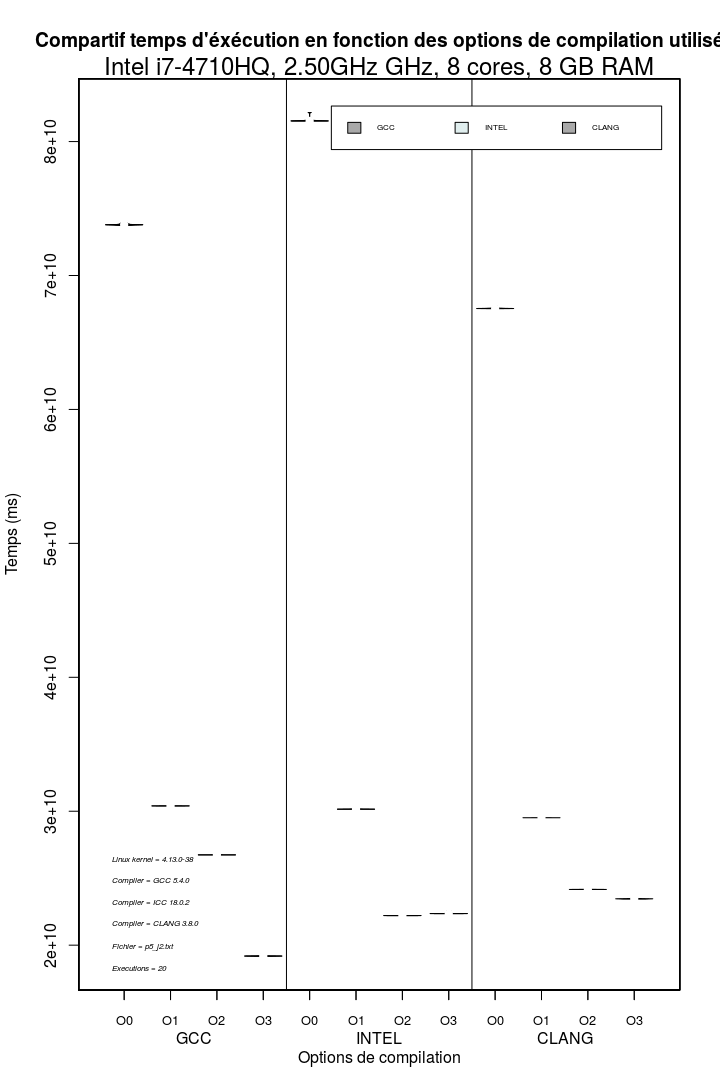
\includegraphics[width=\linewidth, keepaspectratio=true]{GCCvsICCvsCLANG.png}
\end{figure}

\paragraph{Programme Commence}
\begin{figure}[ht]
  \caption{Temps d'exécutions quand le programme commence}
  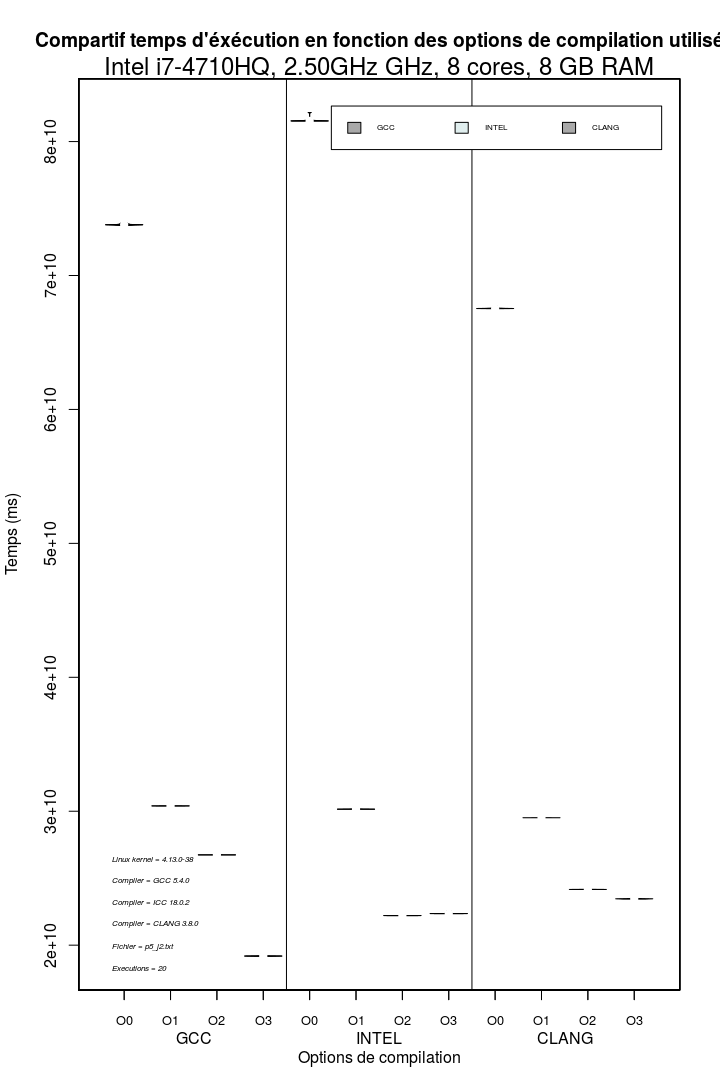
\includegraphics[width=\linewidth, keepaspectratio=true]{GCCvsICCvsCLANG.png}
\end{figure}

\subsubsection{Analyse compilateur par compilateur}
Comme nous l'avons vu précédemment, le fait que le joueur commence ou non n'a pas d'influence sur le choix du compilateur. Nous nous concentrerons dons sur les parties où le programme commence pour analyser plus finement les écarts de temps d'exécutions entre les diverses configurations.\\

\paragraph{GCC}
\begin{figure}[ht]
  \caption{Temps d'exécutions diverses configurations GCC}
  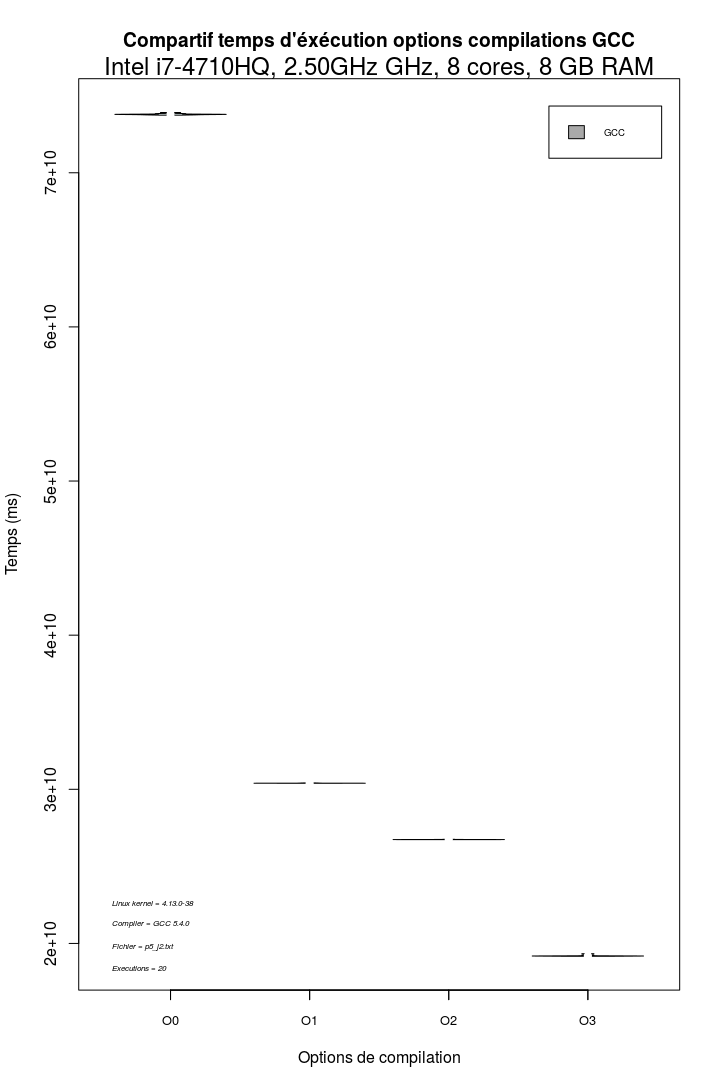
\includegraphics[width=\linewidth, keepaspectratio=true]{GCC.png}
\end{figure}

\paragraph{Intel}
\begin{figure}[ht]
  \caption{Temps d'exécutions diverses configurations Intel}
  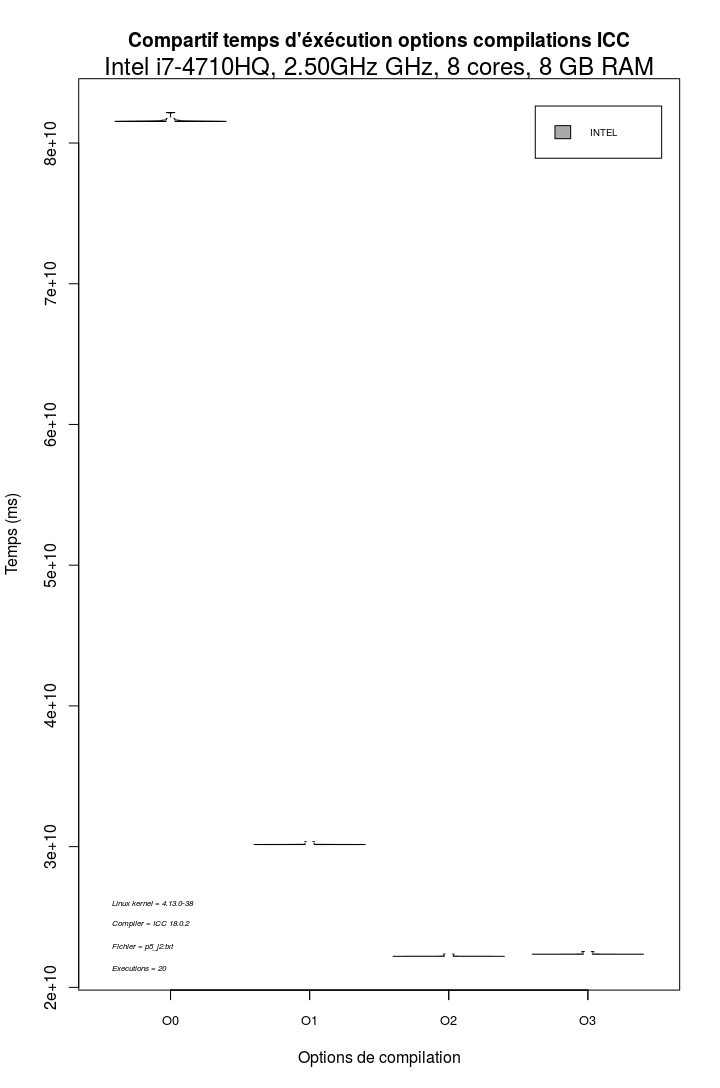
\includegraphics[width=\linewidth, keepaspectratio=true]{ICC.png}
\end{figure}

\paragraph{Clang}
\begin{figure}[ht]
  \caption{Temps d'exécutions diverses configurations Clang}
  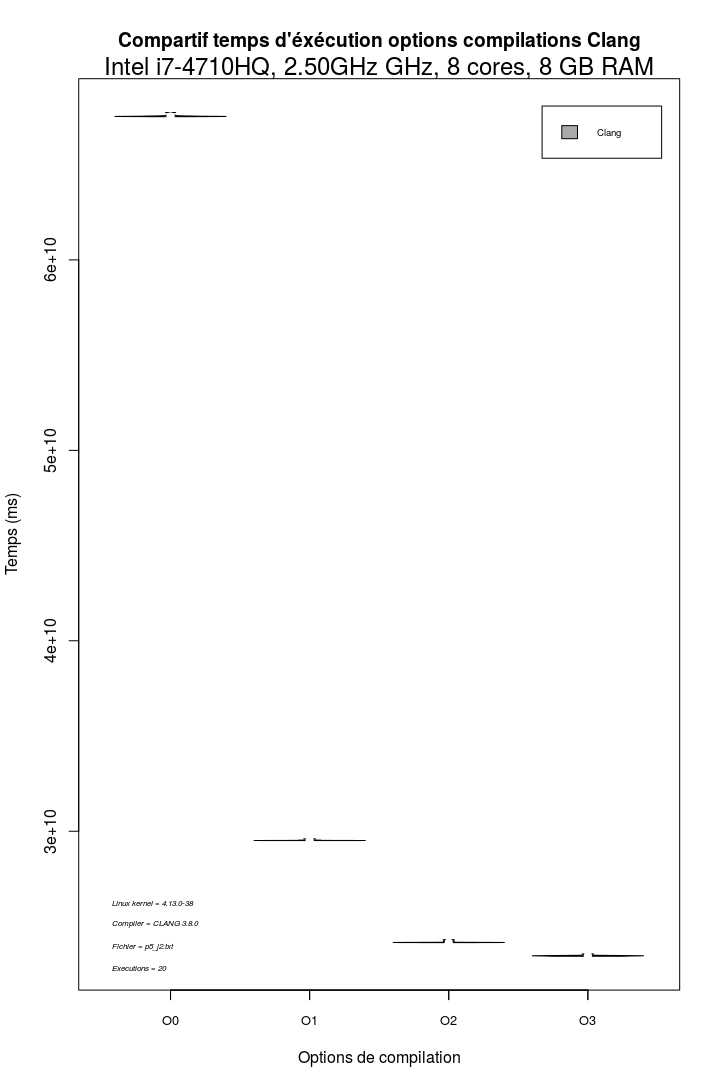
\includegraphics[width=\linewidth, keepaspectratio=true]{CLANG.png}
\end{figure}

\end{document}